\documentclass[preprint,12pt]{elsarticle}

\usepackage{stix}
\usepackage{amsmath,amsthm,mathtools}
\usepackage{booktabs}
\usepackage{enumitem}
\usepackage{graphicx}
\usepackage{lineno}
\usepackage[hidelinks,colorlinks=true,citecolor=blue,linkcolor=red,urlcolor=green,pdfstartview=,pdfauthor=Farshid Mossaiby]{hyperref}

\journal{Neurocomputing}

\newtheorem{definition}{Definition}
\newtheorem{proposition}{Proposition}
\newtheorem{theorem}{Theorem}
\newtheorem{corollary}{Corollary}
\newtheorem{remark}{Remark}

\newcommand{\R}{\mathbb{R}}
\newcommand{\V}{V}
\newcommand{\VBar}{\bar{V}}
\newcommand{\Om}{\Omega}

\setlength{\emergencystretch}{1.5em}

\begin{document}

\begin{frontmatter}

\title{Language Models as Reads over Atom Spaces:\\
A Unified Measure-Theoretic Formulation of Context, Retrieval, and Parameters}

\author[inst1]{Farshid Mossaiby\corref{cor1}}
\ead{mossaiby@eng.ui.ac.ir}
\cortext[cor1]{Corresponding author.}
\affiliation[inst1]{organization={Department of Civil Engineering, University of Isfahan}, postcode={81744-73441}, city={Isfahan}, country={Iran}}

\begin{abstract}
We express finite attention, external retrieval, and expert-output routing through a common read operator: an integral of a query-conditioned measure against a value map over a valued atom space $(\Om,\mathcal F,\nu,v)$. This is an output-space abstraction rather than an assertion that the mechanisms have identical internal computations. We give a sufficient condition for a newly inserted atom to enter an exact top-$k$ set, prove two truncation bounds, and derive an exact-tail rule for selecting the minimum $k$ under a requested error budget. On CounterFact-500, frozen MiniLM exact retrieval obtains 99.2\% rewrite and 91.0\% paraphrase top-1 recall, but a fixed 0.60 activation threshold retains only 38.2\% of paraphrases and falsely activates on 9.6\% of neighborhood prompts. Across five seeds, surface-matched context/corpus/parameter route accuracies are $100.0\pm0.0\%$, $82.4\pm0.9\%$, and $100.0\pm0.0\%$. Matched negative atoms cancel paired signed-read contributions; a perturbation bound and 3000-trial stress test quantify degradation away from exact matching. A ten-fact GPT-2 mechanism study obtains 10/10 canonical and 9/10 paraphrase first-token corrections while ten unrelated controls bypass intervention, compared against a naive fine-tuning baseline and a simplified rank-one (ROME-style) edit at the same ten-fact scale, and against a covariance-regularized ROME reproduction on the full 500-record CounterFact set (85.2\% Efficacy, 59.5\% Paraphrase, 70.1\% Neighborhood Score). These studies do not establish superiority over parametric editing, large-scale ANN performance, certified unlearning, or general factuality improvement.
\end{abstract}

\begin{keyword}
Language models \sep Atom spaces \sep Measure theory \sep External memory \sep Vector retrieval \sep Expert routing
\end{keyword}

\end{frontmatter}

\linenumbers

\section{Introduction}
\label{sec:intro}

Modern autoregressive language models conflate two fundamentally distinct computational roles into dense parameter matrices: general linguistic syntax and factual world knowledge \cite{vaswani2017attention, brown2020language}. While gradient descent is well-suited for acquiring syntactic abstractions, semantic parsing, and structural reasoning, compiling static factual assertions directly into dense weights leads to severe practical bottlenecks. Factual knowledge is dynamic, highly localized, and subject to continuous obsolescence and legal erasure requirements (e.g., the GDPR ``Right to be Forgotten''). When knowledge is frozen within billions of dense parameters, modifying or updating a single fact necessitates expensive retraining or fragile post-hoc weight editing \cite{meng2022locating, meng2023mass}.

To circumvent the rigidity of dense parameter compilation, the community has developed disparate engineering solutions:
\begin{itemize}[leftmargin=1.4em]
  \item \emph{In-context reasoning} stores temporary information in the key-value cache of the sequence window \cite{vaswani2017attention}.
  \item \emph{Retrieval-augmented generation} (RAG) and nearest-neighbor language models ($k$NN-LM) query external vector databases of textual records \cite{lewis2020rag, khandelwal2020generalization, borgeaud2022improving}.
  \item \emph{Modular computation} mechanisms, such as Mixture-of-Experts (MoE) and parameter-efficient adapters (LoRA), route queries across discrete banks of specialized sub-networks \cite{shazeer2017outrageously, hu2021lora, jiang2024mixtral}.
\end{itemize}
Although these techniques share an underlying reliance on key-value similarity matching \cite{geva2021transformer, lample2019large}, they have evolved as disconnected architectural paradigms with distinct mathematical formulations, ad-hoc routing heuristics, and poorly understood stability limits.

In this work, we propose a common measure-theoretic notation for context, external retrieval, and parameter-expert output routing. Attention can be written as an integral of a query-conditioned probability measure against a vector-valued map. Corpus values are fixed records, whereas parameter-expert values may depend on the query; the abstraction identifies their shared weighted-read structure without claiming identical internal computation.

By establishing this equivalence, we make the following contributions:
\begin{enumerate}[leftmargin=1.4em]
  \item \textbf{A Common Mathematical Abstraction:} We formalize the read operator $R(x; \Om)$ and define an integrated tri-space architecture that dynamically arbitrates between context ($\Om_{\mathrm{ctx}}$), corpus retrieval ($\Om_{\mathrm{corpus}}$), and parameter experts ($\Om_{\mathrm{params}}$).
  \item \textbf{A Sufficient Retrieval Condition:} We derive a Lipschitz-margin condition sufficient for a new atom to enter an exact top-$k$ set; prediction success requires additional value and output-margin assumptions.
  \item \textbf{The Quadrature Truncation Bound Theorem:} We prove Theorem~\ref{thm:quadrature_bound}, showing exponential decay of exact ranked top-$k$ truncation error when temperature is calibrated relative to the retrieval gap. ANN candidate quality is a separate approximation not analyzed by the theorem.
  \item \textbf{Signed External-Memory Suppression:} Extending the read to signed reference measures ($\nu = \nu^+ - \nu^-$) permits matched negative atoms to cancel external-memory contributions without retraining; this does not claim removal from pretrained parameters.
  \item \textbf{Controlled Mechanism Studies:} Synthetic and CounterFact experiments examine insertion, adaptive exact truncation, HNSW candidates, cumulative memory, routing, signed-read suppression, and GPT-2 steering. Trainable synthetic studies use five seeds. The implementation and precomputed logs are available at \url{https://github.com/mossaiby/RoAS}.
\end{enumerate}

\section{From a Discrete Function to an Integral}
\label{sec:discrete_to_integral}

\subsection{The Token-Level Function}

A language model is conventionally defined as a conditional probability distribution over a finite vocabulary $\V$ of size $d$, given an input prefix of variable length. To remove indexing dependencies over variable sequence lengths, we fix a maximum context capacity $c$ and introduce a null padding symbol $\varnothing$, yielding an augmented vocabulary $\VBar = \V \cup \{\varnothing\}$. Every input sequence is represented as a fixed-dimensional tuple
\[
  x = (x_1, \dots, x_c) \in \VBar^{\,c},
\]
where unused positions are padded with $\varnothing$. A language model is a mapping
\[
  p : \VBar^{\,c} \to \Delta^{d-1}, \qquad
  \Delta^{d-1} = \Big\{ z \in \R^d : z_i \ge 0,\ \sum_{i=1}^d z_i = 1 \Big\}.
\]

\subsection{Attention as an Integral}

Let $\phi : \VBar \to \R^{e}$ denote a token embedding map such that $\phi(\varnothing) = 0$. We extend the embedded sequence to a step function defined over the continuous interval $[0,c]$:
\[
  f_x(t) = \phi\big(x_{\lceil t \rceil}\big), \qquad t \in (0,c],
\]
with $f_x(0) = \phi(x_1)$. Let \texorpdfstring{$\alpha_x : [0,c] \to \R_{\ge 0}$}{alpha\_x} be a context-dependent attention weight density satisfying the normalization condition $\int_0^c \alpha_x(t)\,dt = 1$, with $\alpha_x(t) = 0$ whenever $x_{\lceil t \rceil} = \varnothing$. We define the aggregate context representation vector as
\[
  z(x) = \int_0^c \alpha_x(t)\, f_x(t)\, dt \in \R^e,
\]
and the corresponding token prediction distribution as
\[
  p(x) = \mathrm{softmax}\big( W z(x) + b \big).
\]
Because $f_x$ is piecewise constant over unit intervals, the continuous integral evaluates algebraically to the standard attention weighted sum \cite{vaswani2017attention, martins2020sparse}:
\[
  \int_0^c \alpha_x(t)\, f_x(t)\, dt = \sum_{i=1}^c \left( \int_{i-1}^i \alpha_x(t)\, dt \right) \phi(x_i) = \sum_{i=1}^c \alpha_i \phi(x_i).
\]
While this establishes algebraic equivalence for standard sequence self-attention, the continuous formulation suggests an immediate generalization: replacing the bounded token coordinate domain $[0,c]$ with an arbitrary, potentially mutable \emph{atom space}.

\section{Atom Spaces: A Common Object for Context, Retrieval, and Parameters}
\label{sec:atomspaces}

\begin{definition}[Valued Atom Space]
A \emph{valued atom space} is a tuple $(\Om, \mathcal{F}, \nu, v)$, where $(\Om,\mathcal{F})$ is a measurable space of elements designated as \emph{atoms}, $\nu$ is a $\sigma$-finite reference measure, and $v : \Om \to \R^e$ is a measurable \emph{value map} into a common output representation space.
\end{definition}

\begin{definition}[Query-Conditioned Kernel and Read Operator]
Given a query $x\in\mathcal X$, let $K_x : \Om \to \R_{\ge 0}$ be measurable and suppose
\[
  0 < Z_x \coloneqq \int_\Om K_x(\omega)\,d\nu(\omega) < \infty.
\]
Then $K_x$ induces a query-conditioned probability measure $\mu_x$ on $(\Om, \mathcal{F})$ via the Radon--Nikodym derivative:
\[
  d\mu_x(\omega) = \frac{K_x(\omega)}{Z_x}\, d\nu(\omega).
\]
If $\int_\Om\|v(\omega)\|_2\,d\mu_x(\omega)<\infty$, the \emph{read} conditioned on $x$ is the Bochner integral:
\[
  R(x; \Om) = \int_\Om v(\omega)\, d\mu_x(\omega) \in \R^e.
\]
\end{definition}

As shown in Table~\ref{tab:instances}, in-context attention, corpus retrieval, and parameter routing are all structural realizations of the read operator $R(x; \Omega)$, differing only in their domain of integration.

\begin{table}[t]
\centering
\caption{Three structural realizations of the unified read operator $R(x; \Omega)$.}
\label{tab:instances}
\vspace{0.5em}
\resizebox{\textwidth}{!}{%
\begin{tabular}{@{}lllll@{}}
\toprule
\textbf{Instance} & \textbf{Atom Space $\Om$} & \textbf{Atom $\omega$} & \textbf{Value Map $v(\omega)$} & \textbf{Operational Equivalent} \\
\midrule
Context & $\{1,\dots,c\}$ & Token index & Embedding $\phi(x_\omega)$ & In-context self-attention \cite{vaswani2017attention} \\
Corpus & $\mathcal{D}$ (mutable) & Factual record & Encoded fact vector & Dense retrieval / $k$NN-LM \cite{khandelwal2020generalization} \\
Parameters & $\Theta$ (expert bank) & Modular expert & Expert output $g_\omega(x)\in\R^e$ & MoE-style output routing \cite{shazeer2017outrageously, hu2021lora} \\
\bottomrule
\end{tabular}%
}
\end{table}

\subsection{The Unified Architecture}

We formulate an integrated architecture where context, external corpus memory, and parameter routing feed into a unified representation:
\[
  z(x) = \lambda_{\mathrm{ctx}}(x) R(x; \Om_{\mathrm{ctx}}) 
       + \lambda_{\mathrm{corpus}}(x) R(x; \Om_{\mathrm{corpus}}) 
       + \lambda_{\mathrm{params}}(x) R(x; \Om_{\mathrm{params}}),
\]
\[
  p(x) = \mathrm{softmax}\big( W_0\, z(x) + b_0 \big),
\]
where $\lambda(x) \in \Delta^2$ is an input-dependent gating distribution across the three spaces, and $W_0 \in \R^{d \times e}, b_0 \in \R^d$ represent the linguistic projection head. For parameter experts the value is query-dependent, $v_x(\omega)=g_\omega(x)$; the read is therefore an output-space mixture, not an average of parameter tensors. Corpus-memory updates can be implemented by inserting, deleting, or reweighting records without changing dense model weights, whereas changing a parameter expert generally requires parameter optimization.

\subsection{System, Calibration, and Tying Principles}

\begin{itemize}[leftmargin=1.4em]
  \item \textbf{Scale Mismatch and Norm Calibration:} The cardinalities of the respective spaces vary across multiple orders of magnitude ($|\Om_{\mathrm{ctx}}| \sim 10^3$, $|\Om_{\mathrm{params}}| \sim 10^1$, $|\Om_{\mathrm{corpus}}| \sim 10^9$). Normalizing a joint softmax across the disjoint union $\Om_{\mathrm{ctx}} \sqcup \Om_{\mathrm{corpus}} \sqcup \Om_{\mathrm{params}}$ causes the largest space to artificially dominate probability mass. Separate intra-space measure normalization combined with calibrated convex gating $\lambda(x)$ is required. Furthermore, key representations across distinct spaces must share identical geometric scales (specifically, unit $L_2$-normalization) to prevent dot-product magnitudes from systematically skewing the router toward higher-norm representations.
  \item \textbf{Tied Value-to-Token Embeddings:} In token generation tasks, the read vector $z_{\mathrm{corpus}}(x)$ should project predictably onto target vocabulary tokens. Letting $E \in \R^{d \times e}$ denote the vocabulary embedding matrix, we use logits $Ez+b$ and values $v(\omega) = E[y_\omega] / \|E[y_\omega]\|$. Isolating atom $\omega^*$ therefore aligns $z(x)$ with the target row. A unique target argmax additionally requires that this alignment exceed the alignment with every competing output row after accounting for bias.
\end{itemize}

\subsection{Signed Atom Spaces and the Hahn--Jordan Decomposition}
\label{sec:signed_spaces}

To support cancellation of external-memory contributions without index reconstruction, we extend the reference measure $\nu$ from a standard non-negative measure to a \emph{signed measure}. By the Hahn--Jordan Decomposition Theorem, any signed reference measure uniquely decomposes into mutually singular non-negative measures:
\[
  \nu = \nu^+ - \nu^-, \qquad \nu^+ \perp \nu^-,
\]
where $\nu^+$ governs positive constructive atoms and $\nu^-$ governs negative ``anti-atoms''. Writing $|\nu|=\nu^++\nu^-$, assume $0<Z_x^{\pm}=\int_\Om K_x\,d|\nu|<\infty$. The normalized signed query measure is
\[
  d\mu_x^{\pm}(\omega) = \frac{K_x(\omega)}{Z_x^{\pm}}\big(d\nu^+(\omega)-d\nu^-(\omega)\big).
\]
This is not a probability measure: its total variation is normalized, while its signed total mass need not equal one. If an anti-atom $\omega^-$ has the same key and value as a positive atom $\omega^*$ and equal positive mass under $\nu^-$ and $\nu^+$, respectively, their contributions cancel exactly inside the signed external read.

\section{Mathematical Conditions for Post-Hoc Knowledge Editing}
\label{sec:editing}

Let the query-key kernel be defined as a scaled inner product:
\[
  K_x(\omega) = \exp\left( \frac{\langle \phi_q(x), \phi_k(\omega) \rangle}{\tau} \right),
\]
where $\phi_q : \mathcal X \to \R^m$ and $\phi_k : \Om \to \R^m$ are query and key encoders, and $\tau > 0$ is a temperature parameter. During base training, $\phi_q$ and $\phi_k$ are optimized against an initial atom pool $\Om_{\mathrm{train}} \subset \Om$. Post-hoc editing requires that inserting a novel, unseen atom $\omega^* \notin \Om_{\mathrm{train}}$ at test time reliably captures the measure $\mu_x(\omega^*)$ for an associated query $x^*$, without modifying the parameters of $\phi_q$ or $\phi_k$.

\subsection{Kernel Locality}

\begin{definition}[Metric Locality]
The key encoder $\phi_k$ is $L$-Lipschitz continuous with respect to a semantic pseudo-metric $d_\Om$ on $\Om$ if
\[
  \| \phi_k(\omega) - \phi_k(\omega') \|_2 \le L\, d_\Om(\omega, \omega') \qquad \forall\, \omega, \omega' \in \Om.
\]
\end{definition}

\begin{proposition}[Score Stability on Unseen Atoms]
\label{prop:score_control}
Let $\phi_k$ be $L$-Lipschitz with respect to $d_\Om$. For any training anchor $\omega_0 \in \Om_{\mathrm{train}}$ and any newly inserted atom $\omega^* \in \Om$, the inner-product similarity score satisfies:
\[
  \big| \langle \phi_q(x), \phi_k(\omega^*) \rangle - \langle \phi_q(x), \phi_k(\omega_0) \rangle \big| 
  \;\le\; \|\phi_q(x)\|_2 \, L \, d_\Om(\omega^*, \omega_0).
\]
\end{proposition}

\begin{proof}
By the Cauchy--Schwarz inequality and the Lipschitz condition:
\begin{align*}
  \big| \langle \phi_q(x), \phi_k(\omega^*) - \phi_k(\omega_0) \rangle \big| 
  &\le \|\phi_q(x)\|_2 \, \|\phi_k(\omega^*) - \phi_k(\omega_0)\|_2 \\
  &\le \|\phi_q(x)\|_2 \, L \, d_\Om(\omega^*, \omega_0). \qedhere
\end{align*}
\end{proof}

\subsection{The Retrieval Margin Condition}

Let $\tau_k(x) = \max^{(k)}_{\omega \in \Om_{\mathrm{train}}} \langle \phi_q(x), \phi_k(\omega) \rangle$ denote the $k$-th highest score among existing training atoms. For the novel atom $\omega^*$ to enter the top-$k$ retrieved set under query $x$, it must satisfy $\langle \phi_q(x), \phi_k(\omega^*) \rangle > \tau_k(x)$. Combining this with Proposition~\ref{prop:score_control} yields a checkable sufficient condition:
\begin{equation}
  \langle \phi_q(x), \phi_k(\omega_0) \rangle - \|\phi_q(x)\|_2 \, L \, d_\Om(\omega^*, \omega_0) \;>\; \tau_k(x),
  \label{eq:margin_condition}
\end{equation}
where $\omega_0$ is a training anchor semantically proximal to $\omega^*$. Equation~\eqref{eq:margin_condition} is a sufficient condition only for top-$k$ inclusion. Successful prediction additionally depends on retrieved probability mass, the value representation, the output margin, and behavior on control queries.

\begin{remark}[The Density--Lipschitz Trade-off]
\label{rem:density_lipschitz}
Equation~\eqref{eq:margin_condition} shows that top-$k$ inclusion depends on both local geometric proximity $d_\Om(\omega^*, \omega_0)$ and the magnitude of $L$. Denser training pools may reduce the distance to a useful anchor, but may also alter encoder norms and competing score margins. Whether density systematically changes the Lipschitz constant is an empirical hypothesis rather than a consequence of the proposition.
\end{remark}

\subsection{Anti-Atoms and Exact External-Read Cancellation}

\begin{proposition}[Matched-Pair Cancellation]
\label{prop:unlearning}
Let an atom $\omega^* \in \Om_{\mathrm{corpus}}$ encode a target fact with tied token value $v^* = E[y^*] / \|E[y^*]\|$. If an anti-atom $\omega^-$ is inserted into the signed atom space with identical key $\phi_k(\omega^-) = \phi_k(\omega^*)$, identical value $v^- = v^*$, and equal positive masses $\nu^-(\{\omega^-\}) = \nu^+(\{\omega^*\})$, then for any query $x$:
\[
  R^{\pm}(x; \{\omega^*, \omega^-\}) = \mathbf{0}.
\]
\end{proposition}

\begin{proof}
Under the signed measure integral of Section~\ref{sec:signed_spaces}, the contribution of the pair evaluates to:
\[
  \int_{\{\omega^*, \omega^-\}} v(\omega)\, d\mu_x(\omega) = \frac{K_x(\omega^*) v^* - K_x(\omega^-) v^*}{Z} = \frac{K_x(\omega^*) (v^* - v^*)}{Z} = \mathbf{0}.
\]
This establishes cancellation of the matched pair's contribution to the signed external read. \qedhere
\end{proof}

Proposition~\ref{prop:unlearning} does not imply that the complete model representation is zero: background atoms, context, parameter experts, residual model states, and output bias may remain. Uniform output follows only in the special case where every other contribution and the output bias are exactly zero. The positive record and anti-atom remain stored, and the proposition does not imply removal of information encoded in pretrained model parameters.

\begin{proposition}[Approximate Pair Cancellation]
\label{prop:approximate_cancellation}
Let $a=K_x(\omega^*)\nu^+(\{\omega^*\})$, $b=K_x(\omega^-)\nu^-(\{\omega^-\})$, and let $Z_x^{\pm}>0$ be the total-variation normalization of the complete signed read. For a positive value $v$ and anti-atom value $\tilde v$, the residual pair contribution satisfies
\[
  \left\|\frac{a v-b\tilde v}{Z_x^{\pm}}\right\|_2
  \le \frac{|a-b|\,\|v\|_2+b\,\|v-\tilde v\|_2}{Z_x^{\pm}}.
\]
\end{proposition}

\begin{proof}
Write $a v-b\tilde v=(a-b)v+b(v-\tilde v)$ and apply the triangle inequality, then divide by $Z_x^{\pm}$. \qedhere
\end{proof}

Thus exact cancellation is sensitive to key-induced kernel mismatch, unequal signed mass, and value mismatch. Query paraphrases affect cancellation only through their effect on the two kernel weights; identical keys still cancel for every query.

\section{Computational Tractability and the Quadrature Truncation Bound}
\label{sec:quadrature}

Evaluating $R(x; \Om) = \int_\Om v(\omega)\, d\mu_x(\omega)$ over a large corpus is expensive if performed densely. We analyze numerical truncation to the exact ranked top-$k$ elements:
\[
  \hat{R}_k(x; \Om) = \sum_{i=1}^k v(\omega_{(i)})\, \frac{K_x(\omega_{(i)})}{\sum_{j=1}^k K_x(\omega_{(j)})}.
\]
The reference implementation computes all $N$ scores and therefore costs $\mathcal{O}(Ne)$ before the top-$k$ read. In deployment, an ANN index may reduce candidate retrieval cost, after which read aggregation costs
\[
  \mathcal{O}(c \cdot e) + \mathcal{O}(k_{\mathrm{corpus}} \cdot e) + \mathcal{O}(k_{\mathrm{params}} \cdot e).
\]
We now formalize the conditions under which this numerical truncation faithfully approximates the continuous integral.

Let $N = |\Om|$, and let $V_{\max} \coloneqq \sup_{\omega \in \Om} \|v(\omega)\|_2 < \infty$. For query $x$, let $s_i \coloneqq \langle \phi_q(x), \phi_k(\omega_i) \rangle$, and let indices be ordered such that $s_{(1)} \ge s_{(2)} \ge \dots \ge s_{(N)}$. Define the normalization terms $Z \coloneqq \sum_{j=1}^N e^{s_{(j)}/\tau}$ and $Z_k \coloneqq \sum_{j=1}^k e^{s_{(j)}/\tau}$. We define the \emph{retrieval spectral gap} at rank $k$ as:
\[
  \Delta_k(x) \coloneqq s_{(1)} - s_{(k+1)} \ge 0.
\]

\begin{theorem}[Quadrature Truncation Error Bound]
\label{thm:quadrature_bound}
For any query $x$ and any truncation depth $k \in \{1, \dots, N-1\}$, the Euclidean approximation error of the top-$k$ quadrature satisfies:
\[
  \| R(x; \Om) - \hat{R}_k(x; \Om) \|_2 \;\le\; 2 V_{\max} \cdot (N - k) \cdot \exp\left( -\frac{\Delta_k(x)}{\tau} \right).
\]
An alternative bound is:
\[
  \| R(x; \Om) - \hat{R}_k(x; \Om) \|_2 \;\le\; 2 V_{\max} \cdot \left(\frac{N - k}{k}\right) \cdot \exp\left( -\frac{s_{(k)} - s_{(k+1)}}{\tau} \right).
\]
\end{theorem}

\begin{proof}
Decompose the difference between the full integral and the top-$k$ truncation:
\begin{align*}
  R(x; \Om) - \hat{R}_k(x; \Om) 
  &= \sum_{i=1}^k v_{(i)} e^{s_{(i)}/\tau} \left( \frac{1}{Z} - \frac{1}{Z_k} \right) + \sum_{i=k+1}^N v_{(i)} \frac{e^{s_{(i)}/\tau}}{Z} \\
  &= \frac{Z_k - Z}{Z Z_k} \sum_{i=1}^k v_{(i)} e^{s_{(i)}/\tau} + \frac{1}{Z} \sum_{i=k+1}^N v_{(i)} e^{s_{(i)}/\tau}.
\end{align*}
Let $Z_{\mathrm{tail}} \coloneqq Z - Z_k = \sum_{i=k+1}^N e^{s_{(i)}/\tau}$. Notice that $\frac{1}{Z_k} \sum_{i=1}^k v_{(i)} e^{s_{(i)}/\tau} = \hat{R}_k(x; \Om)$, and define the tail center of mass $R_{\mathrm{tail}} \coloneqq \frac{1}{Z_{\mathrm{tail}}} \sum_{i=k+1}^N v_{(i)} e^{s_{(i)}/\tau}$. Substituting yields:
\[
  R(x; \Om) - \hat{R}_k(x; \Om) = \frac{Z_{\mathrm{tail}}}{Z} \big( R_{\mathrm{tail}} - \hat{R}_k(x; \Om) \big).
\]
Taking Euclidean norms and applying the triangle inequality:
\[
  \| R(x; \Om) - \hat{R}_k(x; \Om) \|_2 
  \le \frac{Z_{\mathrm{tail}}}{Z} \big( \|R_{\mathrm{tail}}\|_2 + \|\hat{R}_k(x; \Om)\|_2 \big) 
  \le 2 V_{\max} \frac{Z_{\mathrm{tail}}}{Z}.
\]
To bound the tail ratio $\frac{Z_{\mathrm{tail}}}{Z}$, note that $Z \ge e^{s_{(1)}/\tau}$ and $Z_{\mathrm{tail}} = \sum_{i=k+1}^N e^{s_{(i)}/\tau} \le (N - k) e^{s_{(k+1)}/\tau}$:
\[
  \frac{Z_{\mathrm{tail}}}{Z} \;\le\; \frac{(N - k) e^{s_{(k+1)}/\tau}}{e^{s_{(1)}/\tau}} \;=\; (N - k) \exp\left( -\frac{s_{(1)} - s_{(k+1)}}{\tau} \right).
\]
Substituting this into the norm inequality proves the first bound. Alternatively, $Z\ge k e^{s_{(k)}/\tau}$ while $Z_{\mathrm{tail}}\le(N-k)e^{s_{(k+1)}/\tau}$, giving
\[
  \frac{Z_{\mathrm{tail}}}{Z}\le \frac{N-k}{k}\exp\left(-\frac{s_{(k)}-s_{(k+1)}}{\tau}\right),
\]
which proves the second bound. Neither bound uniformly dominates the other; the second is smaller when $s_{(1)}-s_{(k)}<\tau\log k$.
\end{proof}

\begin{corollary}[Error-Budgeted Exact Truncation]
\label{cor:adaptive_k}
Let $\rho_k(x)=Z_{\mathrm{tail}}/Z$ be the exact softmax mass outside the first $k$ ranked atoms. For any requested $\varepsilon>0$, define
\[
  k_\varepsilon(x)=\min\{k\in\{1,\ldots,N\}:2V_{\max}\rho_k(x)\le\varepsilon\}.
\]
Then $\|R(x;\Om)-\hat R_{k_\varepsilon(x)}(x;\Om)\|_2\le\varepsilon$.
\end{corollary}

\begin{proof}
The proof of Theorem~\ref{thm:quadrature_bound} first establishes $\|R-\hat R_k\|_2\le2V_{\max}\rho_k$ before bounding $\rho_k$ by score gaps. Substitution of the defining inequality for $k_\varepsilon(x)$ gives the result. \qedhere
\end{proof}

Theorem~\ref{thm:quadrature_bound} bounds truncation after the exact score ordering is known: when $\tau$ is small relative to $\Delta_k(x)$, the omitted tail decays exponentially. Corollary~\ref{cor:adaptive_k} turns the exact tail mass into a per-query stopping rule, but computing that certificate still requires all scores and therefore is not a sublinear retrieval algorithm. An ANN system introduces an additional candidate-recall error and requires separate empirical evaluation.

\section{Empirical Evaluation}
\label{sec:empirical}

We examine inserted-record retrieval, adaptive exact top-$k$ truncation and scaling, CounterFact retrieval with HNSW candidates, cumulative insertion, tri-space routing, signed-read suppression under perturbation, and GPT-2 steering.

\subsection{Experimental Setup}

\paragraph{Corpus and Domain Design}
We construct a benchmark of 200 structured technical facts distributed equally across four domains: \emph{Astronomy \& Astrophysics}, \emph{Systems \& Computing}, \emph{Chemistry \& Materials Science}, and \emph{Molecular Biology \& Genetics}. Each triplet $(s,r,o)$ is mapped to a declarative record, a canonical query, and one mechanically generated paraphrase. The first 40 items per domain form the adapter-training pool; the remaining 10 items per domain are excluded from adapter training and used as post-hoc insertions. Their labels remain present in the fixed global output vocabulary, making this a transductive label-space evaluation rather than a fully unseen-label split.

\paragraph{Encoder Architecture and Inductive Bias}
We employ a frozen sentence transformer (\texttt{sentence-transformers/all-MiniLM-L6-v2}, $d_{\mathrm{in}} = 384$) as the geometric backbone. To prevent the metric collapse observed when training unconstrained projection heads from scratch on small corpora, we adopt a metric-preserving residual adapter:
\[
  \phi(x) = \mathrm{Normalize}\big( x + 0.1 \cdot \mathrm{MLP}(x) \big),
\]
where the final layer of the MLP is initialized to zero. Values are tied to unit-normalized token embeddings: $v(\omega) = E[y_\omega] / \|E[y_\omega]\|$, with predictions evaluated via the tied projection $p(y \mid x) \propto \langle z(x), E[y] \rangle / \tau$. All engines, benchmark definitions, aggregation scripts, and plotting routines are available at \url{https://github.com/mossaiby/RoAS}.

\paragraph{Reproducibility Environment}
Committed artifacts were generated using Python 3.11.9, PyTorch 2.6.0+cu124, NumPy 2.4.6, sentence-transformers 5.7.0, transformers 4.48.3, and torchvision 0.21.0 on an NVIDIA GeForce RTX 3050 Ti Laptop GPU (4 GB VRAM) with an AMD Ryzen 7 5800U host system and 15.4 GB RAM. Package versions are pinned in \texttt{requirements.txt}. The routing sweep reports seeds $\{40,41,42,43,44\}$ and sample standard deviations; seed 42 is retained as the canonical detailed run. Other experiments use deterministic seed 42.

\subsection{Post-Hoc Knowledge Editing Results}

Table~\ref{tab:editing_triad} compares the trained read with frozen MiniLM exact 1-nearest-neighbor retrieval across pool densities $\Om_{\mathrm{train}} \in \{1, 3, 10, 40\}$ items per domain.

\begin{table}[t]
\centering
\caption{Inserted-record retrieval across 200 templated technical facts. Efficacy and generality denote target classification for a canonical query and one generated paraphrase. Specificity denotes unchanged argmax predictions on active training queries. The adapter spectral product is a diagnostic, not a Lipschitz certificate.}
\label{tab:editing_triad}
\vspace{0.5em}
\resizebox{\textwidth}{!}{%
\begin{tabular}{@{}lcccc@{}}
\toprule
\textbf{Metric} & \textbf{1 / topic} & \textbf{3 / topic} & \textbf{10 / topic} & \textbf{40 / topic} \\
\midrule
\multicolumn{5}{@{}l}{\textit{Trained Residual Read}} \\
Efficacy (Target Recall on $\omega^*$)   & 100.0\%  & 100.0\%  & 100.0\%  & 100.0\%  \\
Generality (Paraphrase Query)           & 100.0\%  & 100.0\%  & 100.0\%  & 100.0\%  \\
Specificity (Neighborhood Retention)    & 100.0\%  & 100.0\%  & 100.0\%  & 100.0\%  \\
\midrule
\multicolumn{5}{@{}l}{\textit{Frozen MiniLM Exact 1-Nearest-Neighbor Baseline}} \\
Efficacy (Target Recall on $\omega^*$)   & 100.0\%  & 100.0\%  & 100.0\%  & 100.0\%  \\
Generality (Paraphrase Query)           & 100.0\%  & 100.0\%  & 100.0\%  & 100.0\%  \\
Specificity (Argmax Retention)          & 100.0\%  & 100.0\%  & 100.0\%  & 100.0\%  \\
\midrule
\multicolumn{5}{@{}l}{\textit{Representation and Metric Dynamics}} \\
Novel Atom Attention Mass $\mu_x(\omega^*)$ & 99.97\%  & 99.97\%  & 99.94\%  & 99.75\%  \\
Adapter Linear Spectral Product         & 0.469    & 0.818    & 0.859    & 1.003    \\
\bottomrule
\end{tabular}%
}
\end{table}

Across the 40 insertion records and all density conditions, both methods obtain 100\% target classification for the canonical query and the single templated paraphrase, with no argmax changes on active training queries. The frozen exact-retrieval baseline therefore matches the trained read: the benchmark does not demonstrate that the residual adapter improves retrieval. At density 40, the trained read's maximum output-probability shift is nonzero ($2.86\times10^{-6}$), showing stability on the evaluated controls rather than zero representational distortion or superiority to parametric editing; competitive baselines such as ROME, MEMIT, WISE, AlphaEdit, and generative RAG are not evaluated here \cite{meng2022locating, meng2023mass, wang2024wise, fang2025alphaedit}.

As training density scales from $1$ to $40$ atoms per domain, the product of the adapter's linear-layer spectral norms increases from $0.469$ to $1.003$, while attention mass decreases from $99.97\%$ to $99.75\%$. This product is a diagnostic of the MLP's linear components, not a certified Lipschitz constant for the complete residual-normalization map $\phi$; directly estimating that constant remains future work.

\subsection{Convergence of Exact Ranked \texorpdfstring{Top-$k$}{Top-k} Truncation}

Table~\ref{tab:truncation_error} presents the empirical quadrature truncation error $\| R_{\mathrm{exact}}(x) - \hat{R}_k(x) \|_2 = \| z_{\mathrm{exact}}(x) - z_k(x) \|_2$ across temperatures and cutoffs $k$ on the largest atom pool (density 40, containing 160 active background atoms).

\begin{table}[t]
\centering
\caption{Quadrature truncation error $\| R_{\mathrm{exact}} - \hat{R}_k \|_2$ evaluated on context vectors across temperatures $\tau$ and retrieval cutoffs $k$. Under unit-normalized embeddings ($V_{\max}=1$), error is strictly bounded by $2.0$ and exhibits exponential decay at sharp operational temperatures ($\tau = 0.05, k=1 \implies 3.82 \times 10^{-6}$).}
\label{tab:truncation_error}
\vspace{0.5em}
\resizebox{\textwidth}{!}{%
\begin{tabular}{@{}lccccc@{}}
\toprule
\textbf{Temperature} & \textbf{Top-1} & \textbf{Top-3} & \textbf{Top-5} & \textbf{Top-10} & \textbf{Top-20} \\
\midrule
$\tau = 0.05$ & $3.82 \times 10^{-6}$ & $3.01 \times 10^{-6}$ & $2.62 \times 10^{-6}$ & $2.03 \times 10^{-6}$ & $1.41 \times 10^{-6}$ \\
$\tau = 0.10$ & $0.0182$ & $0.0170$ & $0.0162$ & $0.0145$ & $0.0121$ \\
$\tau = 0.50$ & $0.965$ & $0.700$ & $0.558$ & $0.384$ & $0.245$ \\
$\tau = 1.00$ & $0.988$ & $0.623$ & $0.477$ & $0.327$ & $0.217$ \\
\bottomrule
\end{tabular}%
}
\end{table}

The numerical results illustrate the temperature dependence of exact truncation. We also compute both theorem bounds for every query. At density 40, $\tau=0.10$, and $k=1$, the maximum observed error is $0.0244$ and the smaller pointwise bound covers 100\% of queries with minimum slack $0.0923$. This checks the implemented inequalities in this finite numerical setting rather than establishing bound tightness or ANN behavior:
\begin{itemize}[leftmargin=1.4em]
  \item \textbf{Concentration at Low Temperatures (\texorpdfstring{$\tau = 0.05$}{tau = 0.05}):} At the operational reading temperature, the mean error for $k=1$ is $3.82 \times 10^{-6}$, decaying to $1.41 \times 10^{-6}$ at $k=20$. In this benchmark, the query measure is concentrated almost entirely on the nearest scored records.
  \item \textbf{Diffuse Measure Truncation at High Temperatures (\texorpdfstring{$\tau \ge 0.50$}{tau >= 0.50}):} When the kernel temperature is uncalibrated, probability mass spreads broadly across background atoms, producing truncation errors approaching $1.0$. Exact top-$k$ truncation is therefore faithful only when paired with sharp, metric-calibrated kernels.
\end{itemize}

\paragraph{Adaptive error budgets and scaling}
We additionally evaluate Corollary~\ref{cor:adaptive_k} on 64 correlated synthetic queries with unit-normalized random keys and values in $\R^{128}$, for $N\in\{1000,5000,10000,25000\}$. Across both temperatures and all three budgets $\varepsilon\in\{0.01,0.05,0.10\}$, every measured read error satisfies its certificate (100\% empirical coverage). The result also exposes conservatism: at $N=25{,}000$ and $\varepsilon=0.05$, mean $k_\varepsilon$ is $13{,}026$ (52.1\% of the corpus) for $\tau=0.05$ and $21{,}467$ (85.9\%) for $\tau=0.10$. Exact scoring, sorting, and reading take 54.6 and 18.2 ms, respectively, on the reported GPU run. Thus the rule provides a checkable accuracy budget but does not guarantee a small $k$ for diffuse or weakly separated score distributions.

\subsection{CounterFact External-Memory Retrieval and ANN Candidates}
\label{sec:counterfact}

We evaluate the frozen MiniLM retrieval geometry on the first 500 CounterFact records introduced with ROME~\cite{meng2022locating}. Each external-memory key is the benchmark rewrite prompt concatenated with its requested new target; evaluation uses 500 rewrite prompts, the first two paraphrases per record (1000 queries), and the first two neighborhood prompts (1000 queries). This is an external-memory retrieval experiment, not a parametric editing comparison with ROME or MEMIT.

\begin{table}[t]
\centering
\caption{CounterFact-500 external-memory retrieval. ``Activated correct'' applies cosine threshold 0.60 after exact top-1 retrieval. Neighborhood activation is undesirable. HNSW candidate recall asks whether its ten candidates contain the exact top-1.}
\label{tab:counterfact_retrieval}
\vspace{0.5em}
\resizebox{\textwidth}{!}{%
\begin{tabular}{@{}lcc@{}}
\toprule
\textbf{Evaluation} & \textbf{Metric} & \textbf{Result} \\
\midrule
Rewrite prompts & Exact top-1 / activated correct & 99.2\% / 99.2\% \\
Paraphrase prompts & Exact top-1 / activated correct & 91.0\% / 38.2\% \\
Neighborhood prompts & False activation / paired wrong-edit retrieval & 9.6\% / 2.4\% \\
Adaptive read ($\varepsilon=0.05$) & Mean $k$ / maximum error / coverage & 246.0 / 0.0237 / 100\% \\
Fixed read ($k=10$) & Mean / maximum vector error & 0.1769 / 0.4461 \\
HNSW, 10 candidates & Exact top-1 candidate recall & 99.96\% \\
\bottomrule
\end{tabular}
}
\end{table}

Table~\ref{tab:counterfact_retrieval} shows that pretrained embedding geometry retrieves most corresponding records, but the fixed threshold rejects a majority of otherwise-correct paraphrase matches. A FAISS HNSW index obtains 99.96\% exact-top-1 candidate recall in this 500-record run, with 12.7 ms construction and 23.5 ms search for all 2500 queries. These timings are implementation- and hardware-specific, and the corpus is too small to establish large-scale ANN behavior.

\subsection{CounterFact-Scale Parametric Editing: ROME at 500 Records}
\label{sec:counterfact_rome}

The ten-fact ROME-lite baseline in Section~\ref{sec:generative} shares scale with the naive fine-tuning baseline but not with the 500-record CounterFact retrieval evaluation above. To close that gap, we implement a second, more faithful ROME reproduction~\cite{meng2022locating} directly on the same 500 CounterFact records used in Table~\ref{tab:counterfact_retrieval}. Three changes bring it closer to the original method than the ten-fact ROME-lite baseline: (i) the key/value association is inserted at the record's actual subject span, located via tokenizer offset mapping, rather than the final prompt token; (ii) a single edit layer is selected once via a lightweight causal trace (embedding corruption plus per-layer MLP restoration) averaged over 50 held-out records (disjoint from evaluation), matching how the original method fixes one layer per model rather than searching per edit; and (iii) the closed-form rank-one update uses a genuine key covariance matrix $C=\mathbb{E}[kk^{\top}]$, estimated over every token position of 1500 held-out CounterFact generation/attribute texts (also disjoint from evaluation and from the layer-selection sample) at the selected layer, in place of the identity-covariance approximation: $W\leftarrow W + (C^{-1}k)(v^*-k^{\top}W)^{\top}/(k^{\top}C^{-1}k)$. This substitutes in-repository held-out text for the Wikipedia sample used by the original implementation, avoiding a new external download dependency. It remains simplified relative to the original paper in two respects: a single canonical prompt per record (no multi-template key averaging) and a plain teacher-forced cross-entropy objective for $v^*$ (no KL ``essence'' regularizer). We report the standard CounterFact Efficacy, Paraphrase, and Neighborhood Scores~\cite{meng2022locating}, each compared as first-sub-token probability of the new versus true target rather than mean log-probability over the full multi-token target, plus the same control-text perplexity ratio used elsewhere in this paper.

\begin{table}[t]
\centering
\caption{CounterFact-500 ROME reproduction on GPT-2 (124M) with a genuine key-covariance prior and real subject spans, versus the ten-fact naive fine-tuning and ROME-lite baselines from Table~\ref{tab:finetune_baseline}. Efficacy/Paraphrase/Neighborhood Scores compare first-sub-token target-new versus target-true probability, following the original CounterFact metric definitions at reduced (single-template, no-KL-regularizer) fidelity.}
\label{tab:counterfact_rome}
\vspace{0.5em}
\resizebox{\textwidth}{!}{%
\begin{tabular}{@{}lccc@{}}
\toprule
\textbf{Metric} & \textbf{Naive FT (10 facts)} & \textbf{ROME-Lite (10 facts)} & \textbf{ROME, CounterFact-500} \\
\midrule
Efficacy Score & 100\% (argmax) & 100\% (argmax) & 85.2\% (35.6\% argmax) \\
Paraphrase Score & 70\% (argmax) & 40\% (argmax) & 59.5\% \\
Neighborhood Score / specificity & 58.9\% (mean) & 87.8\% (mean) & 70.1\% \\
Control-text perplexity ratio & 0.982 mean, 1.022 max & 0.996 mean, 1.004 max & 1.001 mean, 1.291 max \\
Edit layer(s) & All parameters & Per-record (mostly layer 10/12) & Single global layer 3/12 \\
\bottomrule
\end{tabular}%
}
\end{table}

At CounterFact-500 scale, the covariance-regularized ROME reproduction obtains an 85.2\% Efficacy Score (35.6\% exact first-token argmax; the probability-based score is more permissive because it only requires the new target to outrank the true target, not to be the single most likely continuation), a 59.5\% Paraphrase Score, and a 70.1\% Neighborhood Score, with control-text perplexity essentially unchanged on average (1.001) but a 1.291 worst-case ratio on at least one edited record. These numbers are well below the published full-fidelity ROME results on larger GPT-2 variants, consistent with the disclosed simplifications (single-template keys, no KL regularizer, a smaller 124M-parameter model, and an in-repository covariance corpus rather than a Wikipedia sample); they are not a like-for-like reproduction of the original paper's reported numbers. They do, however, extend the specificity/generality trade-off observed in the ten-fact comparison to literature scale: relative to the ten-fact ROME-lite baseline, moving to real subject spans, a fixed globally-selected layer, and covariance regularization raises paraphrase generality (40\%$\to$59.5\%) while giving up some neighborhood specificity (87.8\%$\to$70.1\%), which is directionally consistent with the original paper's own ablation showing that covariance regularization trades some specificity for broader generalization relative to an identity-covariance update.

\subsection{Lifelong Cumulative Knowledge Editing Benchmark}
\label{sec:lifelong}

To evaluate whether the atom-space formulation provides lifelong memory stability, we conduct a cumulative insertion experiment:
\begin{enumerate}[leftmargin=1.4em]
  \item We train the base model on 160 baseline atoms (initial accuracy: 100.0\%).
  \item We insert all 40 held-out technical facts \emph{sequentially and permanently without teardown}, expanding the active pool from 161 to 200 atoms.
  \item At regular intervals, we evaluate Cumulative Efficacy across all facts inserted up to that point, Cumulative Generality across paraphrases, Background Specificity across the original 160 training facts, and the Mean Attention Mass $\mu_x(\omega^*)$ allocated to the target atoms.
\end{enumerate}

Table~\ref{tab:lifelong_editing} and Figure~\ref{fig:lifelong_curve} present the results of this lifelong evaluation.

\begin{table}[t]
\centering
\caption{Cumulative insertion performance across 40 sequential records without teardown. Target argmax recall and training-query argmax agreement remain $100.0\pm0.0\%$ across five seeds.}
\label{tab:lifelong_editing}
\vspace{0.5em}
\resizebox{\textwidth}{!}{%
\begin{tabular}{@{}lcccccc@{}}
\toprule
\textbf{Sequential Edits Inserted} & \textbf{1} & \textbf{5} & \textbf{10} & \textbf{20} & \textbf{30} & \textbf{40} \\
\textbf{Total Active Pool Size} & \textbf{161} & \textbf{165} & \textbf{170} & \textbf{180} & \textbf{190} & \textbf{200} \\
\midrule
Cumulative Efficacy (All Past Edits)   & 100.0\% & 100.0\% & 100.0\% & 100.0\% & 100.0\% & 100.0\% \\
Cumulative Generality (Paraphrases)    & 100.0\% & 100.0\% & 100.0\% & 100.0\% & 100.0\% & 100.0\% \\
Background Specificity (Original 160)  & 100.0\% & 100.0\% & 100.0\% & 100.0\% & 100.0\% & 100.0\% \\
Mean Attention Mass $\mu_x(\omega^*)$  & 99.84\% & 99.76\% & 99.46\% & 99.60\% & 99.66\% & 99.70\% \\
\bottomrule
\end{tabular}%
}
\end{table}

\begin{figure}[t]
\centering
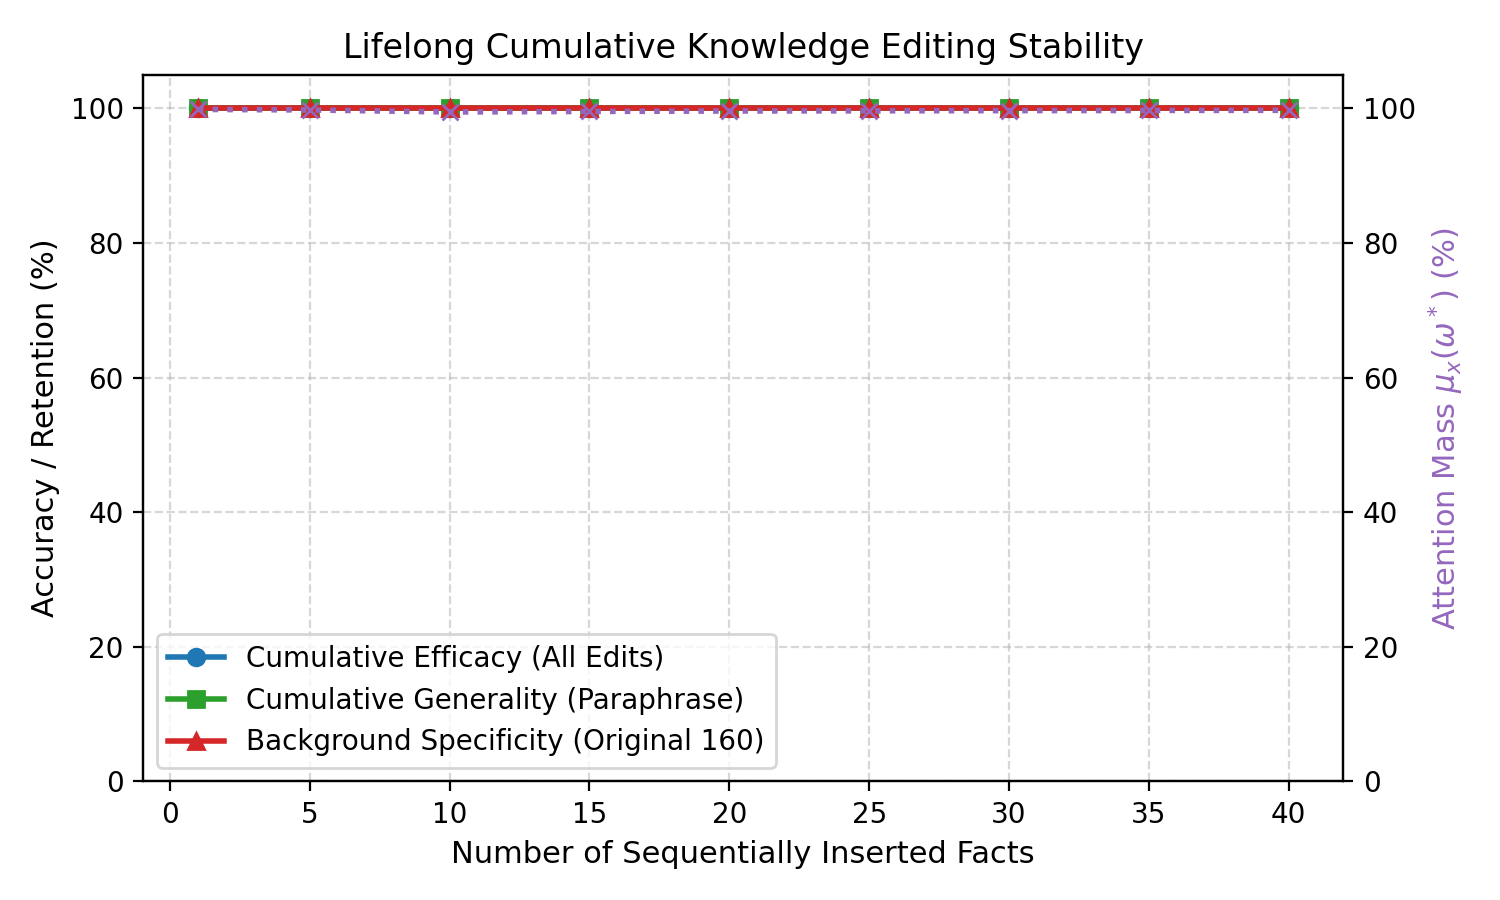
\includegraphics[width=0.72\linewidth]{figures/lifelong_retention_curve.png}
\caption{Lifelong cumulative knowledge editing stability across 40 sequential fact insertions. Cumulative efficacy, generality, and background specificity remain perfectly stable at 100\%, while the query-conditioned attention probability mass $\mu_x(\omega^*)$ remains tightly concentrated at $>99.6\%$ despite continuous memory expansion.}
\label{fig:lifelong_curve}
\end{figure}

Across five seeds, all 39 earlier insertions remain correctly classified when the 40th record is added, and no argmax changes are observed on the 160 training queries. At 40 insertions, mean target-atom attention mass is $99.681\pm0.014\%$. These observations apply to this small exact-scoring benchmark; the truncation theorem does not itself prove resistance to forgetting or memory dilution.

\subsection{Dynamic Tri-Space Routing and Path Ablation}
\label{sec:trigating}

To evaluate the integrated tri-space architecture of Section~\ref{sec:atomspaces}, we construct an empirical environment with three task domains assigned to different information paths:
\begin{enumerate}[leftmargin=1.4em]
  \item \textbf{In-Context Ephemeral Reasoning ($\Om_{\mathrm{ctx}}$):} Input sequences provide ad-hoc premises unavailable in world memory (e.g., synthetic cryptographic bindings). The model must attend to local token positions $\Om_{\mathrm{ctx}}$.
  \item \textbf{Corpus World Knowledge ($\Om_{\mathrm{corpus}}$):} Prompts ask declarative technical questions from our factual repository without providing premise context. The model must route to $\Om_{\mathrm{corpus}}$.
  \item \textbf{Parameter-Resident Expert Outputs ($\Om_{\mathrm{params}}$):} Queries describe small procedural classification tasks. Trigger keys select trainable, unit-normalized expert vectors stored as model parameters rather than corpus values.
\end{enumerate}

The tri-space router $\lambda(x) \in \Delta^2$ is parameterized as a lightweight projection network trained jointly with the representation heads. To prevent the norm scale mismatch analyzed in Section~\ref{sec:atomspaces}, parameter-expert keys are normalized to the unit sphere, matching the geometric scale of the corpus embeddings. Evaluation uses unseen query strings with the identical wrapper ``Determine the output for:'' across all three families, removing explicit route words such as ``premise,'' ``stored,'' and ``expert.''

\begin{table}[t]
\centering
\caption{Five-seed surface-matched routing and ablation (mean $\pm$ sample standard deviation). Route accuracy is the fraction whose largest gate selects the intended space. Tasks and labels are known during training, but evaluation strings are unseen and share one wrapper across families.}
\label{tab:tri_space_gating}
\vspace{0.5em}
\resizebox{\textwidth}{!}{%
\begin{tabular}{@{}lcccccc@{}}
\toprule
\textbf{Task Domain} & \textbf{Task Acc.} & \textbf{Route Acc.} & \multicolumn{3}{c}{\textbf{Mean Gating Distribution $\lambda(x)$}} & \textbf{Ablated Acc.} \\
\cmidrule(lr){4-6}
& & & $\lambda_{\mathrm{ctx}}$ & $\lambda_{\mathrm{corpus}}$ & $\lambda_{\mathrm{params}}$ & \\
\midrule
In-Context Reasoning ($\Omega_{\mathrm{ctx}}$) & $100.0{\pm}0.0$ & $100.0{\pm}0.0$ & $\mathbf{68.0{\pm}2.1}$ & $6.2{\pm}0.9$ & $25.8{\pm}1.3$ & $0.0{\pm}0.0$ \\
Corpus World Knowledge ($\Omega_{\mathrm{corpus}}$) & $96.8{\pm}1.8$ & $82.4{\pm}0.9$ & $12.9{\pm}0.7$ & $\mathbf{56.6{\pm}2.2}$ & $30.5{\pm}1.7$ & $0.0{\pm}0.0$ \\
Parameter Expert Outputs ($\Omega_{\mathrm{params}}$) & $100.0{\pm}0.0$ & $100.0{\pm}0.0$ & $3.1{\pm}0.2$ & $3.1{\pm}0.4$ & $\mathbf{93.7{\pm}0.5}$ & $0.0{\pm}0.0$ \\
\bottomrule
\end{tabular}%
}
\end{table}

\begin{figure}[t]
\centering
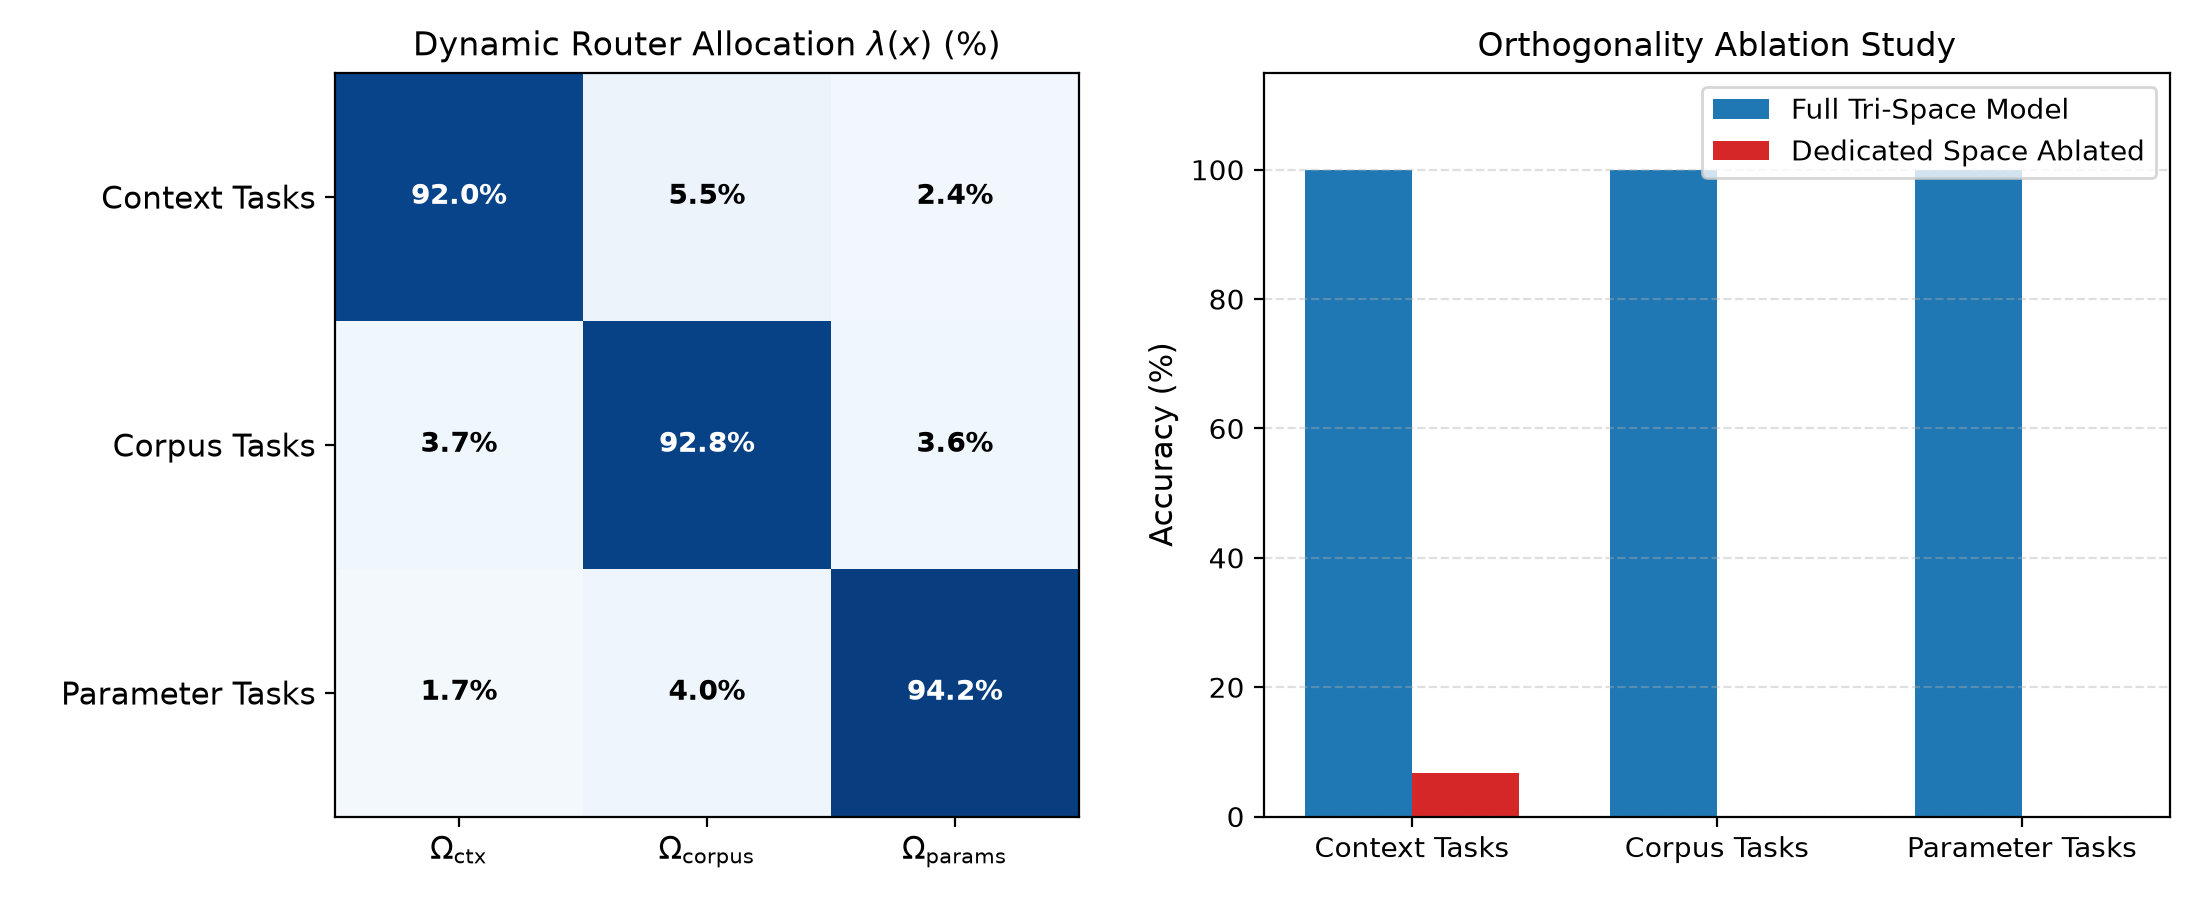
\includegraphics[width=0.88\linewidth]{figures/tri_space_gating_ablation.png}
\caption{Five-seed surface-matched tri-space evaluation. Left: mean router allocation on unseen strings with a shared wrapper. Right: mean task accuracy with sample-standard-deviation error bars; intended-path ablation reduces accuracy to zero.}
\label{fig:tri_space_ablation}
\end{figure}

Table~\ref{tab:tri_space_gating} and Figure~\ref{fig:tri_space_ablation} present the surface-matched results:
\begin{itemize}[leftmargin=1.4em]
  \item \textbf{Routing Generalization:} Mean route accuracy is $100.0\%$, $82.4\%$, and $100.0\%$ for context, corpus, and parameter tasks. Mean intended-space allocation is $68.0\%$, $56.6\%$, and $93.7\%$, respectively.
  \item \textbf{Task and Ablation Results:} Mean full-model accuracy is $100.0\%$, $96.8\%$, and $100.0\%$; ablating the intended space reduces every corresponding accuracy to 0\% in all five runs.
\end{itemize}
Removing explicit route words exposes partial corpus confusion with the parameter path. These results establish limited surface-form robustness over the same records, operations, and labels. They do not establish transfer to held-out task families, expert composition, or adversarial robustness.

\subsection{Knowledge Contradiction and Anti-Atom External-Memory Suppression}
\label{sec:unlearning}

In practical applications, external-memory records may require correction or suppression. We examine both operations in a controlled signed-read classifier; we do not evaluate physical deletion, privacy guarantees, or removal from pretrained parameters.

\paragraph{External-Memory Suppression via Anti-Atoms}
To test zero-retraining suppression in the external read, five synthetic sensitive records are inserted into the base corpus. Without gradient descent or index reconstruction, we insert an anti-atom $\omega^-$ with positive mass $1.0$ under $\nu^-$ and value $v^- = E[y_{\mathrm{sensitive}}]$ at the same metric coordinate as each record. This benchmark evaluates matched-query output suppression, not certified deletion from pretrained weights.

\begin{table}[t]
\centering
\caption{External-memory suppression and counterfactual updating via signed reads, using a toy 49-token output vocabulary. Exact matched pairs reduce target probability to approximately $1/|\mathcal{V}|=2.04\%$ in this external-read-only classifier. Clean-control argmax accuracy remains 100.0\%.}
\label{tab:unlearning_results}
\vspace{0.5em}
\resizebox{\textwidth}{!}{%
\begin{tabular}{@{}lcccc@{}}
\toprule
\textbf{Target Entity / Query} & \textbf{Pre-Edit P(Target)} & \textbf{Post-Edit P(Target)} & \textbf{Status} & \textbf{Background Specificity} \\
\midrule
\multicolumn{5}{@{}l}{\textit{External-Memory Suppression via Anti-Atoms (unit mass under $\nu^-$)}} \\
Secret Base Alpha Coordinates   & 99.998\% & \textbf{2.04\%} ($1/|\mathcal{V}|$) & Suppressed & 100.0\% \\
Patient Confidential Diagnosis  & 99.998\% & \textbf{2.04\%} ($1/|\mathcal{V}|$) & Suppressed & 100.0\% \\
Proprietary Patent Number       & 99.998\% & \textbf{2.04\%} ($1/|\mathcal{V}|$) & Suppressed & 100.0\% \\
Classified Document Location    & 99.998\% & \textbf{2.04\%} ($1/|\mathcal{V}|$) & Suppressed & 100.0\% \\
VIP Cryptographic Key           & 99.998\% & \textbf{2.04\%} ($1/|\mathcal{V}|$) & Suppressed & 100.0\% \\
\midrule
\multicolumn{5}{@{}l}{\textit{Counterfactual Competitive Updating ($w_{\mathrm{new}} = 2.5$, Append-Only)}} \\
Ethereum $\to$ Proof-of-Stake   & 3.0\% (old) & \textbf{40.0\%} (new) & Overridden & 100.0\% \\
Java $\to$ Oracle               & 0.01\% (old)& \textbf{60.1\%} (new) & Overridden & 100.0\% \\
Pluto $\to$ Dwarf Planet        & 32.3\% (old)& 23.9\% (new)          & Competing  & 100.0\% \\
Twitter $\to$ X Corp            & 99.8\% (old)& 0.04\% (new)          & Lexical Bias & 100.0\% \\
Python $\to$ PyPy JIT           & 98.9\% (old)& 0.24\% (new)          & Lexical Bias & 100.0\% \\
\bottomrule
\end{tabular}%
}
\end{table}

\begin{figure}[t]
\centering
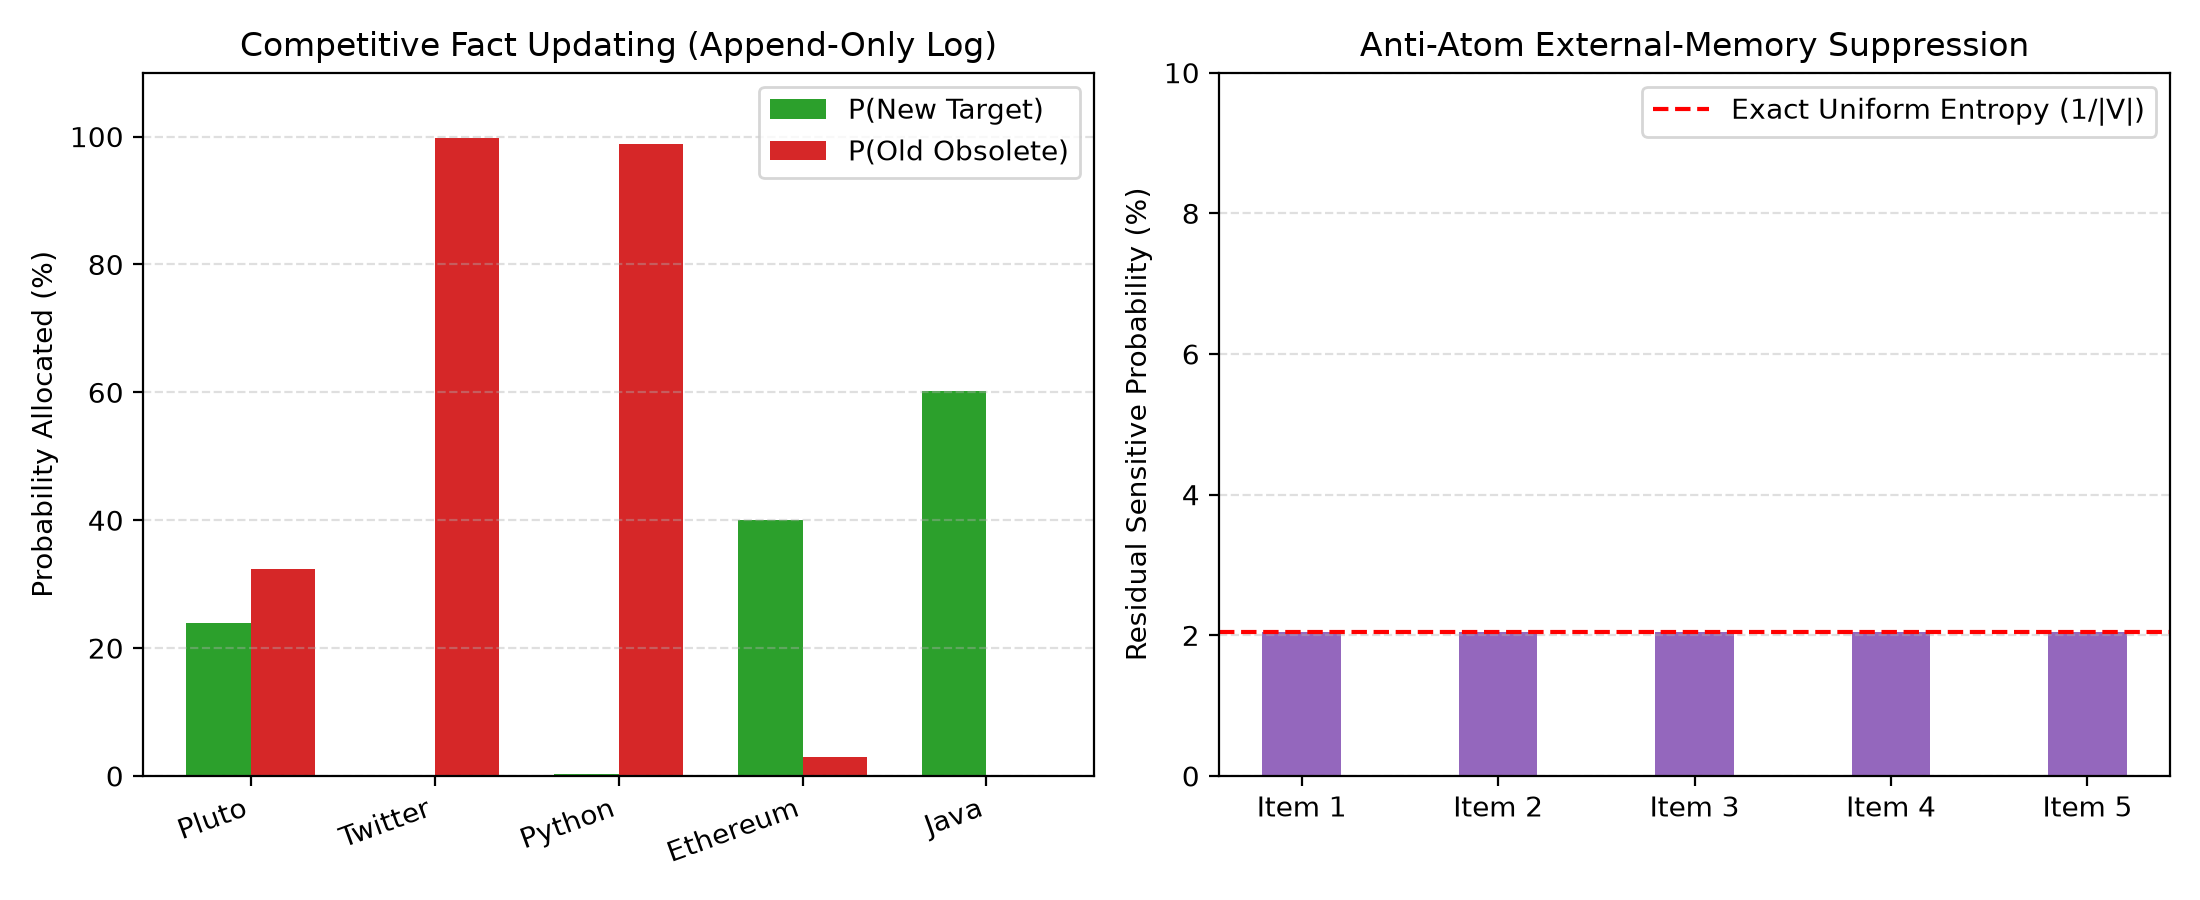
\includegraphics[width=0.88\linewidth]{figures/unlearning_and_updates.png}
\caption{Empirical evaluation of signed atom spaces. Left: Competitive counterfactual updating in an append-only log under passive recency weighting ($w_{\mathrm{new}} = 2.5$). Right: matched anti-atom cancellation drives residual target probability to uniform entropy ($P = 2.04\% \approx 1/|\mathcal{V}|$) in the external read.}
\label{fig:unlearning_plots}
\end{figure}

Table~\ref{tab:unlearning_results} and Figure~\ref{fig:unlearning_plots} (right) show that matched anti-atoms reduce target-token probability to approximately \textbf{2.04\%}. In a vocabulary of $|\V|=49$ tokens, $1/49\approx0.0204$. The paired contribution is exactly zero by construction; small background contributions remain in the complete read. Argmax accuracy on 35 clean control facts remains \textbf{100.0\%}.

\paragraph{Approximate cancellation stress test}
We next perturb the anti-atom key, value, mass, or query over 50 random trials at magnitudes 0, 0.01, 0.05, 0.10, and 0.20, with background sizes 10, 100, and 1000. The analytical bound covers all 3000 trials. At $N=100$, key perturbations of 0.01, 0.05, and 0.10 leave mean pair residuals of 4.5\%, 72.1\%, and 98.0\% relative to the original positive contribution; corresponding value perturbations leave 5.5\%, 25.5\%, and 40.5\%, while 1\%, 5\%, and 10\% mass errors leave 0.5\%, 2.4\%, and 4.8\%. Query perturbation alone leaves numerical-zero residual because both exactly matched keys receive the same changed kernel weight. Exact anti-atoms are therefore algebraically effective but fragile to key mismatch.

\paragraph{Competitive Updating and the Lexical Bias Phenomenon}
In an append-only log where old atoms cannot be physically deleted, we evaluate updating five technical statements by inserting contradictory atoms $\omega_{\mathrm{new}}$ with priority recency weighting $w_{\mathrm{new}} = 2.5$.
Across five seeds, competitive updating succeeds on $44.0\pm8.9\%$ of the five records per run; the canonical seed succeeds for two records (\emph{Ethereum $\to$ Proof-of-Stake} and \emph{Java $\to$ Oracle}). In the remaining canonical cases, similarity to the old key outweighs the fixed recency weight under the exponential kernel. Matched anti-atom suppression succeeds on $100.0\pm0.0\%$ of records, with mean residual probability $2.0407\pm0.00002\%$ and $100.0\pm0.0\%$ background specificity.

This small result shows that a fixed passive recency weight is not sufficient for every evaluated update. Active cancellation is one possible design response, but broader benchmarks are required before selecting an update policy.

\subsection{Autoregressive Generative Modeling with GPT-2}
\label{sec:generative}

To establish that the atom-space read operator functions effectively in multi-layer causal generative architectures, we hook $\Om_{\mathrm{corpus}}$ directly into the final hidden representation of a pretrained transformer (\texttt{gpt2}, 124M parameters \cite{radford2019language}).

\paragraph{Continuous Hidden-State Augmentation with Relevance Gating}
At each greedy decoding step $t$, the current textual prefix $x_{1:t}$ is encoded by the frozen sentence encoder, $q_t = \phi_q(x_{1:t}) \in \R^m$, and matched against the corpus atom space. GPT-2 independently maps the token prefix to $h_t \in \R^{d_{\mathrm{model}}}$. A matching atom is injected only if its cosine score exceeds 0.60 and it has not already been consumed in the current generation. This one-shot rule prevents repeated injection of the same target token:
\[
  \tilde{h}_t =
  \begin{cases}
    (1-\lambda_{\mathrm{read}})h_t+\lambda_{\mathrm{read}}W_{\mathrm{proj}}z_t,
      & \text{relevant and unconsumed},\\
    h_t, & \text{otherwise}.
  \end{cases}
\]
feeding directly into the language model head: $p(x_{t+1} \mid x_{1:t}) = \mathrm{softmax}(W_{\mathrm{LM}} \tilde{h}_t)$. Each atom's value $v_i$ is mapped to the token embedding of the target entity from GPT-2's vocabulary matrix.

\begin{table}[t]
\centering
\caption{Selected rows from a ten-fact greedy GPT-2 (124M) evaluation. Factual atoms boost first-token target probabilities and flip all ten canonical first predictions.}
\label{tab:generative_results}
\vspace{0.5em}
\resizebox{\textwidth}{!}{%
\begin{tabular}{@{}lccccc@{}}
\toprule
\textbf{Factual Target Task} & \multicolumn{2}{c}{\textbf{Target Probability $P(y^*)$}} & \textbf{Ratio} & \multicolumn{2}{c}{\textbf{Top Predicted Token}} \\
\cmidrule(lr){2-3} \cmidrule(lr){5-6}
& \textbf{Base GPT-2} & \textbf{Atom-Space} & & \textbf{Base GPT-2} & \textbf{Atom-Space} \\
\midrule
QUIC Transport Protocol (\texttt{UDP})         & 2.64\% & \textbf{70.00\%} & 26.5$\times$   & \texttt{the}     & \textbf{\texttt{UDP}} \\
Milky Way Black Hole (\texttt{Sagittarius})    & 0.47\% & \textbf{64.33\%} & 136.3$\times$  & \texttt{after}   & \textbf{\texttt{Sag}} \\
Safe Systems Language (\texttt{Rust})          & 0.03\% & \textbf{32.99\%} & 1116.0$\times$ & \texttt{a}       & \textbf{\texttt{Rust}} \\
Uranium Radiative Decay (\texttt{lead})        & 0.87\% & \textbf{9.80\%}  & 11.3$\times$   & \texttt{uranium} & \textbf{\texttt{lead}} \\
CRISPR Bacterial Defense (\texttt{viruses})    & 2.25\% & \textbf{38.41\%} & 17.1$\times$   & \texttt{infect.} & \textbf{\texttt{viruses}} \\
\bottomrule
\end{tabular}%
}
\end{table}

\begin{figure}[t]
\centering
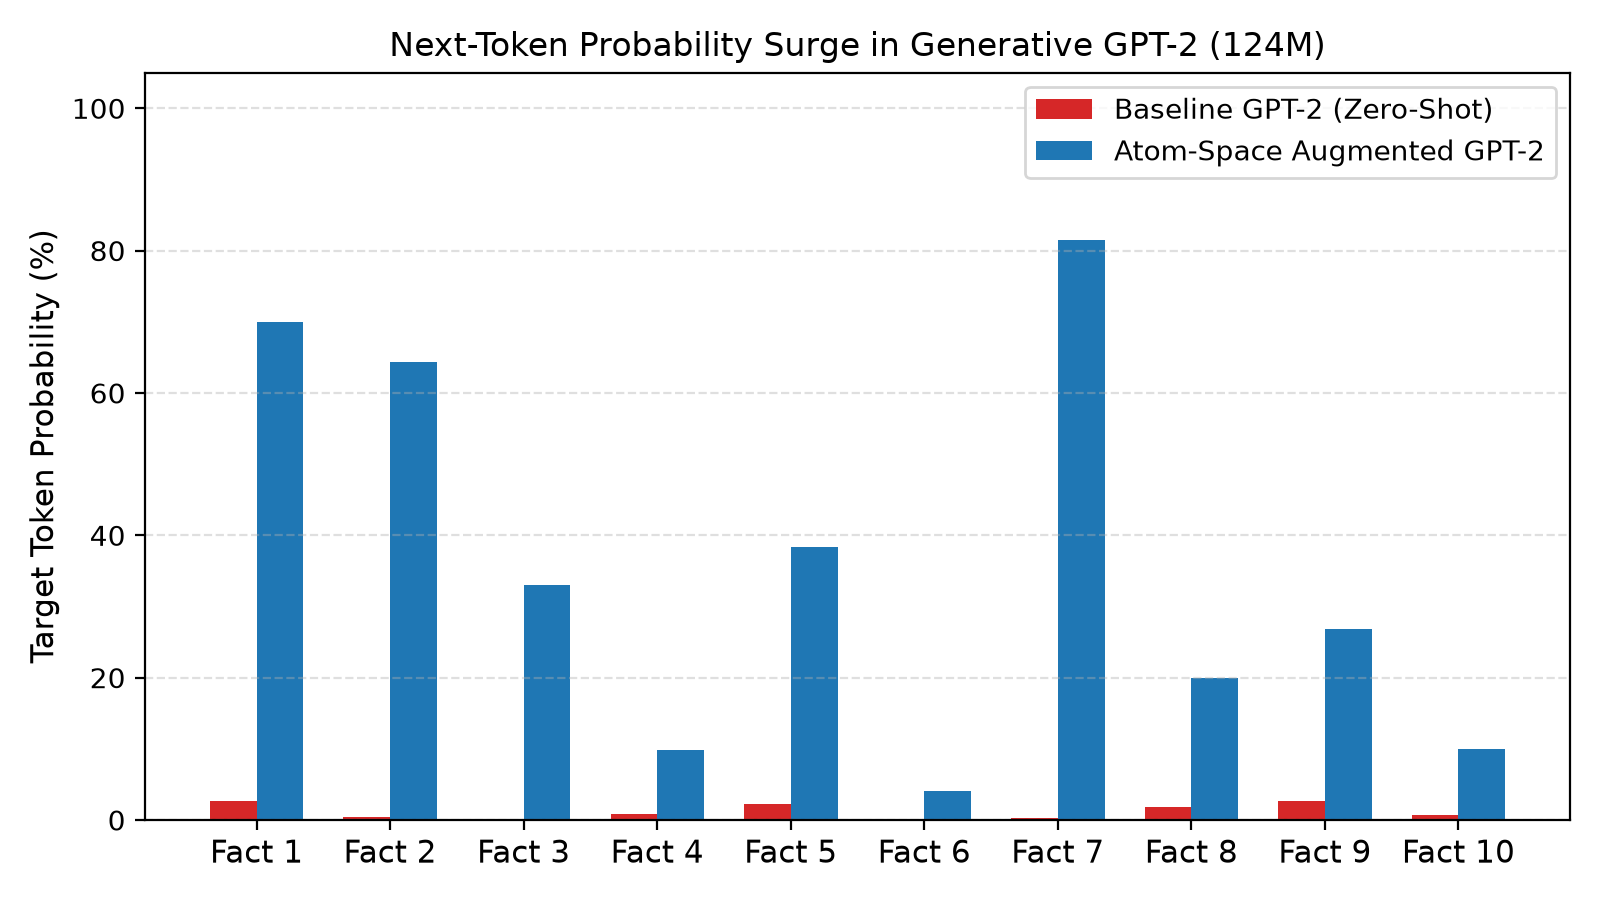
\includegraphics[width=0.72\linewidth]{figures/generative_probability_boost.png}
\caption{First-token target probabilities in GPT-2 (124M) before and after direct target-embedding intervention. The argmax changes toward the desired first token or subtoken on all five selected prompts.}
\label{fig:generative_boost}
\end{figure}

\paragraph{First-Token Correction and Multi-Token Continuation}
Table~\ref{tab:generative_results} and Figure~\ref{fig:generative_boost} summarize the quantitative performance. Base GPT-2 assigns $<3\%$ probability to the correct factual token in all cases, generating severe hallucinations upon free autoregressive decoding:
\begin{itemize}[leftmargin=1.4em]
  \item \textbf{Milky Way Black Hole Prompt:} Base GPT-2 generates: \emph{``The supermassive black hole at the center of the Milky Way is named \textbf{after the famous astronomer Johannes Kepler, who discovered the black hole\dots}''}. The intervention changes the first generated subtoken from \texttt{after} to \texttt{Sag} ($0.47\% \to 64.33\%$ target probability), and the tokenizer completes ``Sagittarius A'' before the continuation later becomes unreliable.
  \item \textbf{Uranium Decay Prompt:} Base GPT-2 generates \emph{``natural uranium decays radiatively into stable isotopes of \textbf{uranium\dots}''}. The intervention changes the first generated token to \texttt{lead} ($0.87\% \to 9.80\%$), but the later phrase ``lead, thorium, and lead-based materials'' is not a reliable scientific continuation.
  \item \textbf{Systems Language Prompt:} Base GPT-2 generates generic filler: \emph{``The systems programming language offering memory safety without garbage collection is \textbf{a great way to get around the limitations\dots}''} Augmented with the atom space, probability surges by $1116\times$ ($0.03\% \to 32.99\%$), generating: \emph{``The systems programming language offering memory safety without garbage collection is \textbf{Rust. The Rust compiler is a powerful tool for\dots}''}
\end{itemize}
Across all ten canonical prompts, the intervention changes the first-token argmax to the desired token or subtoken. Teacher-forced scoring over complete target strings obtains 96.7\% target-token accuracy, reflecting one later-subtoken error for ``chloroplast.'' On ten manually constructed paraphrases, retrieval selects the intended atom and changes the first-token argmax on 9/10. Across ten unrelated control texts, the similarity threshold prevents activation at every teacher-forced step, so the augmented/base perplexity ratio is exactly 1.0 by construction. A grid over thresholds $\{0.4,0.5,0.6,0.7,0.8\}$ and $\lambda_{\mathrm{read}}\in\{0.25,0.5,0.75,0.85\}$ records factual and false activation separately. These tests remain too small to establish naturalness, broad language preservation, or factuality gains.

\paragraph{Naive Full-Parameter Fine-Tuning Baseline}
To give the atom-space read a first parametric point of comparison, we fine-tune all of GPT-2's parameters on each of the ten canonical facts in isolation: starting from the pretrained checkpoint, we take gradient steps (AdamW, learning rate $10^{-5}$, up to 25 steps, early-stopped at training loss $<0.01$) on the canonical prompt-target pair, then reset to the clean checkpoint before the next fact. This is the standard unconstrained ``FT'' baseline from the model-editing literature.

\paragraph{ROME-Lite: A Simplified Locate-and-Edit Baseline}
We additionally implement a simplified, single-layer rank-one edit in the style of ROME~\cite{meng2022locating} on the same ten facts, so all three methods share identical prompts, paraphrases, neighborhood facts, and control texts. For each fact we (i) select an edit layer among $\{2,4,6,8,10\}$ via a lightweight single-token causal trace (Gaussian corruption of the final prompt token's embedding, then per-layer MLP restoration, keeping the layer with the largest probability recovery); (ii) take the key $k$ as the clean model's MLP down-projection input at that token and optimize a value $v^*$ with teacher-forced cross-entropy only (20 Adam steps, no KL ``essence'' regularizer); and (iii) insert the association with the closed-form identity-covariance rank-one update $W \leftarrow W + k\,(v^*-k^{\top}W)^{\top}/(k^{\top}k)$ to the down-projection weight. This omits ROME's multi-template key averaging, precomputed key-covariance statistics, and KL regularization against a separate prompt set, and is evaluated at the same ten-fact scale as the fine-tuning baseline; it is a same-scale, same-metric comparison point, not a reproduction of ROME's published numbers.

\begin{table}[t]
\centering
\caption{Naive full-parameter fine-tuning and a simplified single-layer rank-one edit (ROME-lite) versus the relevance-gated atom-space read on the same ten GPT-2 facts, paraphrases, and control texts. Neighborhood specificity has no atom-space analogue because the read injects no weight changes.}
\label{tab:finetune_baseline}
\vspace{0.5em}
\resizebox{\textwidth}{!}{%
\begin{tabular}{@{}lccc@{}}
\toprule
\textbf{Metric} & \textbf{Atom-Space Read} & \textbf{Naive Fine-Tuning (FT)} & \textbf{ROME-Lite} \\
\midrule
Canonical efficacy (first-token argmax) & 100\% (10/10) & 100\% (10/10) & 100\% (10/10) \\
Paraphrase generality (first-token argmax) & 90\% (9/10) & 70\% (7/10) & 40\% (4/10) \\
Neighborhood specificity (other 9 facts' argmax unchanged) & n/a (no weight change) & 58.9\% (mean) & 87.8\% (mean) \\
Control-text perplexity ratio (locality) & 1.000 (exact, by construction) & 0.982 mean, 1.022 max & 0.996 mean, 1.004 max \\
Mechanism & Relevance-gated read, zero weight updates & Full-parameter gradient descent, mean 18.0 steps/fact & Single-layer rank-one edit, identity-covariance closed form \\
\bottomrule
\end{tabular}%
}
\end{table}

Table~\ref{tab:finetune_baseline} shows that naive fine-tuning matches the atom-space read's canonical efficacy but generalizes less well to paraphrases (70\% vs.\ 90\%) and, more importantly, changes the argmax on 41.1\% of the other nine facts' canonical queries on average even though each fact is edited in isolation and training loss converges below 0.01. Mean control-text perplexity drifts by up to 2.2\% in the worst case, whereas the atom-space read leaves unrelated text perplexity exactly unchanged because unrelated prompts never cross the activation threshold. ROME-lite's single-layer, identity-covariance edit reduces neighborhood argmax drift substantially relative to full-parameter fine-tuning (12.2\% vs.\ 41.1\% of other facts changed) and keeps control-text perplexity closer to the pre-edit model (0.4\% mean drift vs.\ 1.8\%), consistent with the locality benefits reported for locate-and-edit methods in the literature. However, at this simplified, single-template scale it generalizes to paraphrases substantially worse than either the fine-tuning baseline or the atom-space read (40\% vs.\ 70\% and 90\%), plausibly because omitting ROME's multi-template key averaging leaves the inserted association keyed too tightly to the single canonical prompt's representation. This three-way, same-scale comparison illustrates both the catastrophic-interference risk that motivates locate-and-edit methods and the specificity/generality trade-off between them, but remains restricted to ten facts on GPT-2 (124M) with a simplified, non-covariance-regularized edit; a full-fidelity reproduction of ROME, MEMIT, WISE, or AlphaEdit at CounterFact scale \cite{meng2022locating, meng2023mass, wang2024wise, fang2025alphaedit} remains future work.

\section{Discussion and Related Work}
\label{sec:discussion}

The individual components unified under our framework have extensive histories in machine learning:
\begin{itemize}[leftmargin=1.4em]
  \item \textbf{Retrieval and Memory Networks:} $k$NN-LM \cite{khandelwal2020generalization}, RETRO \cite{borgeaud2022improving}, and Memory Networks \cite{sukhbaatar2015end, lample2019large} correspond directly to the corpus read $R(x; \Om_{\mathrm{corpus}})$.
  \item \textbf{Parameter Routing and Mixture-of-Experts:} MoE models \cite{shazeer2017outrageously, fedus2022switch, jiang2024mixtral} and dynamic LoRA routing \cite{hu2021lora} represent realizations of $R(x; \Om_{\mathrm{params}})$, where expert selection reflects a discrete, sparse measure over parameter patches.
  \item \textbf{In-Context Attention:} Standard multi-head attention \cite{vaswani2017attention} is an integral $R(x; \Om_{\mathrm{ctx}})$ over discrete sequence indices.
\end{itemize}

What this formulation contributes beyond existing empirical literature is fivefold:
\begin{enumerate}[leftmargin=1.4em]
  \item \textbf{A Common Mathematical Object:} By expressing context, corpus retrieval, and parameter routing as integrals over measurable atom spaces, these mechanisms can be analyzed within a unified framework. Surface-matched evaluation quantifies both successful routing and corpus-to-parameter confusion.
  \item \textbf{A Checkable Retrieval Condition:} The Lipschitz-margin inequality gives a sufficient condition for exact top-$k$ inclusion. It is not by itself a guarantee of edit success, generalization, or specificity.
  \item \textbf{A Quadrature Foundation for Vector Retrieval:} Theorem~\ref{thm:quadrature_bound} and Corollary~\ref{cor:adaptive_k} link the read integral to exact ranked truncation and error-budgeted $k$. HNSW candidate recall is measured separately~\cite{malkov2020hnsw}.
  \item \textbf{Cumulative External-Memory Insertion:} External records are additive over the measured atom space ($\Om_t=\Om_0\cup\{\omega^*\}$). In the 200-record experiment, no argmax changes are observed on training controls. Section~\ref{sec:generative} adds two ten-fact parametric comparison points: a naive full-parameter fine-tuning baseline that matches canonical efficacy but shows weaker paraphrase generality and substantial neighborhood drift, and a simplified single-layer rank-one edit (ROME-lite) that recovers most of that lost neighborhood specificity while generalizing to paraphrases worse than either alternative. Section~\ref{sec:counterfact_rome} extends this to a covariance-regularized ROME reproduction \cite{meng2022locating} at the same 500-record CounterFact scale used for retrieval, obtaining a 59.5\% Paraphrase Score and 70.1\% Neighborhood Score at reduced (single-template, no-KL-regularizer) fidelity. A full-fidelity comparison against MEMIT \cite{meng2023mass} and recent lifelong or null-space-constrained editors \cite{wang2024wise, fang2025alphaedit} at CounterFact scale is left for future work.
  \item \textbf{Zero-Retraining External-Memory Suppression:} Signed reads enable matched anti-atoms to cancel selected external-memory contributions without weight retraining or index reconstruction.
\end{enumerate}

Finally, our generative experiment applies relevance-gated atom reads throughout greedy decoding, demonstrating first-token factual steering without fine-tuning.

\subsection{Limitations}
The trainable synthetic studies use five seeds but remain small and templated. Frozen exact 1-nearest-neighbor retrieval matches the trained read on synthetic insertions. CounterFact retrieval uses only 500 records and does not compare end-to-end generation against MEMIT, MEND, WISE, AlphaEdit, or RAG \cite{meng2023mass, wang2024wise, fang2025alphaedit}. Three parametric editing comparison points are provided at increasing fidelity and scale: a naive full-parameter fine-tuning baseline and a ten-fact single-layer rank-one (ROME-lite) baseline (Section~\ref{sec:generative}), and a covariance-regularized ROME reproduction \cite{meng2022locating} on the full 500-record CounterFact evaluation set (Section~\ref{sec:counterfact_rome}). All three remain simplified relative to the original ROME implementation: a single canonical prompt per record rather than multi-template key averaging, no KL ``essence'' regularizer during value optimization, first-sub-token rather than full multi-token target probability comparisons, and (for the CounterFact-scale version) an in-repository held-out text corpus rather than a Wikipedia sample for covariance estimation. None reproduce ROME's originally published numbers, which were obtained on larger GPT-2 variants. Exact adaptive certification computes all pairwise scores; its large selected fractions show that it is not itself a scaling solution. The HNSW corpus is too small for large-scale latency conclusions. Tri-space tasks and labels are known during training, and parameter experts are output vectors rather than subnetworks or LoRA patches. Anti-atoms retain both records and do not remove pretrained knowledge; key mismatch rapidly weakens cancellation, and extraction/privacy attacks are not evaluated. The GPT-2 study has ten facts, ten paraphrases, and ten controls, so it remains a mechanism study rather than evidence of general hallucination reduction.

\section{Conclusion}
\label{sec:conclusion}

We have presented a measure-theoretic abstraction that casts finite attention, dense retrieval, and parameter-expert output routing as weighted reads into a common output space. We derived a sufficient condition for top-$k$ inclusion, exact-ranked truncation bounds, an adaptive error-budget rule, and an approximate cancellation bound, then examined them in controlled synthetic and CounterFact studies.

The synthetic insertion studies obtain perfect five-seed target classification and retention, but frozen exact 1-nearest-neighbor retrieval obtains the same result. Error-budgeted exact truncation achieves complete empirical coverage while often requiring a large fraction of the corpus. CounterFact reveals strong exact retrieval but weak fixed-threshold paraphrase activation and nonzero neighborhood activation; HNSW recovers the exact top-1 among ten candidates in this small run. The remaining studies show imperfect routing, fragile approximate cancellation, and limited GPT-2 factual-token steering. Competitive end-to-end baselines, larger corpora and models, held-out task families, privacy attacks, and broad language evaluations remain necessary before comparative performance claims.

\section*{CRediT Authorship Contribution Statement}
\textbf{Farshid Mossaiby}: Conceptualization, Methodology, Formal analysis, Software, Investigation, Validation, Data curation, Writing - original draft, Writing - review \& editing.

\section*{Declaration of Competing Interest}
The author declares that they have no known competing financial interests or personal relationships that could have appeared to influence the work reported in this paper.

\section*{Data Availability}
The complete open-source codebase, synthetic and technical benchmarks, experimental suites, and reproduction scripts generated during this study are publicly available in the GitHub repository at \url{https://github.com/mossaiby/RoAS}.

\section*{Declaration of Generative AI in Scientific Writing}
During the preparation of this work, the author utilized Google Gemini to assist in the mathematical formalization of quadrature bounds, experimental pipeline design, and manuscript formatting. After using this tool, the author reviewed and edited the content as needed and takes full responsibility for the content of the publication.

\bibliographystyle{elsarticle-num}
\bibliography{references}

\end{document}